\section{}
% An incompressible Newtonian liquid is confined between two concentric circular 
% cylinders of infinite length – a solid inner cylinder of radius 𝑅𝑖 and a hollow, 
% stationary outer cylinder of radius 𝑅𝑜. The inner cylinder rotates at angular 
% velocity 𝜔𝑖
% . The flow is steady, laminar, and two-dimensional in the 𝑟𝜃-plane. 
% The flow is also rotationally symmetric, meaning that nothing is a function of 
% coordinate 𝜃 (𝑢𝜃 and 𝑃 are functions of radius 𝑟 only). The flow is also circular, 
% meaning that velocity component 𝑢𝑟 = 0 everywhere. Generate an exact 
% expression for velocity component 𝑢𝜃 as a function of radius 𝑟 and the other 
% parameters in the problem. You may ignore gravity.

\textit{An incompressible Newtonian liquid is confined between two concentric circular cylinders of infinite length – a solid inner cylinder of radius $R_i$ and a hollow, stationary outer cylinder of radius $R_o$. The inner cylinder rotates at angular velocity $\omega_i$. The flow is steady, laminar, and two-dimensional in the $r\theta$-plane. The flow is also rotationally symmetric, meaning that nothing is a function of coordinate $\theta$ ($u_{\theta}$ and $P$ are functions of radius $r$ only). The flow is also circular, meaning that velocity component $u_r = 0$ everywhere. Generate an exact expression for velocity component $u_{\theta}$ as a function of radius $r$ and the other parameters in the problem. You may ignore gravity.}

\begin{figure}[h]
    \centering
    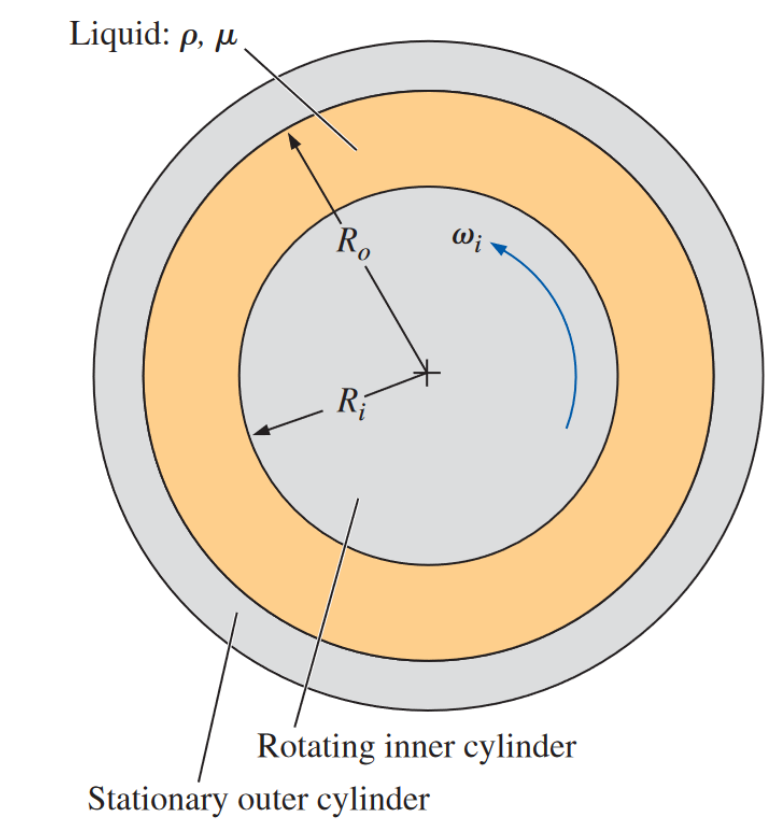
\includegraphics[width=0.5\textwidth]{Questions/Figures/Q2 Problem Diagram.png}
\end{figure}
\FloatBarrier
\subsection*{Solution}
First we list our assumptions and their consequences:
\begin{table}[h]
    \centering
    \begin{tabular}{ccc}
        \toprule
        Number & Assumption & Consequence \\
        \hline
        \#1 & Steady flow & $\frac{\partial}{\partial t} = 0$ \\
        \#2 & Incompressible flow & $\rho = \text{constant}$ \\
        \#3 & Two-dimensional flow & $u_z = 0$, $\partial_z \vec{v} = 0$ \\
        \#4 & No Gravity on $r$, $\theta$ & $g_r = g_{\theta} = 0$ \\
        \#5 & Rotationally Symmetric Flow & $u_{\theta} = u_{\theta}(r)$, $P = P(r)$ \\
        \#6 & Circular Flow & $u_r = 0$ \\
        \bottomrule
    \end{tabular}
\end{table}
Also note the boundary conditions:
\begin{align*}
    u_{\theta}(R_i) &= R_i \omega_i \\
    u_{\theta}(R_o) &= 0
\end{align*}
Starting with the continuity equation, we have
\begin{align*}
    \frac{1}{r} \frac{\partial (r u_r)}{\partial r} + \frac{1}{r} \cancelto{\text{\#5}}{\frac{\partial u_{\theta}}{\partial \theta}} + \cancelto{\text{\#3}}{\frac{\partial u_z}{\partial z}} = 0
\end{align*}
Now the momentum equation in the $\theta$ direction is
% use the underbrace form
% $\theta$ & \(\displaystyle \begin{aligned} \frac{\partial u_{\theta}}{\partial t} + u_r \frac{\partial u_{\theta}}{\partial r} + \frac{u_{\theta}}{r} \frac{\partial u_{\theta}}{\partial \theta} + \frac{u_r u_{\theta}}{r} + u_z \frac{\partial u_{\theta}}{\partial z} &= -\frac{1}{\rho r} \frac{\partial P}{\partial \theta} + g_{\theta} \\ &\quad + \frac{\mu}{\rho} \biggr[\underbrace{\frac{1}{r} \frac{\partial}{\partial r}\left(r \frac{\partial u_{\theta}}{\partial r}\right) - \frac{u_{\theta}}{r^2}}_{\displaystyle \frac{\partial}{\partial r}\left(\frac{1}{r}\frac{\partial}{\partial r}(r u_{\theta})\right)} + \frac{1}{r^2} \frac{\partial^2 u_{\theta}}{\partial \theta^2} + \frac{2}{r^2} \frac{\partial u_{\theta}}{\partial \theta} + \frac{\partial^2 u_{\theta}}{\partial z^2}\biggr] \end{aligned}\) \\[9ex]
\begin{align*}
    \cancelto{\text{\#1}}{\frac{\partial u_{\theta}}{\partial t}} + \cancelto{\text{\#6}}{u_r \frac{\partial u_{\theta}}{\partial r}} + \frac{u_{\theta}}{r} \cancelto{\text{\#5}}{\frac{\partial u_{\theta}}{\partial \theta}} + \cancelto{\text{\#6}}{\frac{u_r u_{\theta}}{r}} + u_z \cancelto{\text{\#3}}{\frac{\partial u_{\theta}}{\partial z}} &= -\frac{1}{\rho r} \cancelto{\text{\#5}}{\frac{\partial P}{\partial \theta}} + \cancelto{\text{\#4}}{g_{\theta}} \\
    &\quad + \frac{\mu}{\rho} \left[\frac{\partial}{\partial r}\left(\frac{1}{r}\frac{\partial}{\partial r}(r u_{\theta})\right) + \frac{1}{r^2} \cancelto{\text{\#5}}{\frac{\partial^2 u_{\theta}}{\partial \theta^2}} + \frac{2}{r^2} \cancelto{\text{\#5}}{\frac{\partial u_{\theta}}{\partial \theta}} + \cancelto{\text{\#3}}{\frac{\partial^2 u_{\theta}}{\partial z^2}}\right]
\end{align*}
which simplifies to
\begin{align*}
    \frac{\partial}{\partial r}\left(\frac{1}{r}\frac{\partial}{\partial r}(r u_{\theta})\right) &= 0
\end{align*}
Integrating,
\begin{align*}
    \frac{1}{r}\frac{\partial}{\partial r}(r u_{\theta}) &= C_1 \\
    \frac{\partial}{\partial r}(r u_{\theta}) &= C_1 r \\
    r u_{\theta} &= \frac{1}{2} C_1 r^2 + C_2 \\
    u_{\theta} &= \frac{1}{2} C_1 r + \frac{C_2}{r}
\end{align*}
Applying the boundary conditions,
\begin{align*}
    u_{\theta}(R_o) &= 0 = \frac{1}{2} C_1 R_o + \frac{C_2}{R_o} \implies C_2 = -\frac{1}{2} C_1 R_o^2 \\
    u_{\theta}(R_i) &= R_i \omega_i = \frac{1}{2} C_1 R_i + \frac{C_2}{R_i} \implies R_i \omega_i = \frac{1}{2} C_1 R_i - \frac{1}{2} C_1 \frac{R_o^2}{R_i}
\end{align*}
Solving,
\begin{align*}
    \implies R_i \omega_i &= C_1 \left(\frac{R_i}{2} - \frac{R_o^2}{2R_i}\right) \\
    \implies C_1 &= \frac{2 R_i^2 \omega_i}{R_i^2 - R_o^2} \\
    \implies C_2 &= \frac{R_i^2 R_o^2 \omega_i}{R_o^2 - R_i^2}
\end{align*}
Thus,
\begin{align*}
    u_{\theta} &= \frac{R_i^2 \omega_i}{R_i^2 - R_o^2} r + \frac{R_i^2 R_o^2 \omega_i}{R_o^2 - R_i^2} \frac{1}{r} \\
    \Aboxed{&= \left(\frac{R_i^2 \omega_i}{R_o^2 - R_i^2}\right) \left(\frac{R_o^2}{r} - r\right)}
\end{align*}
